\documentclass[11pt]{article}
 
\usepackage{fancyhdr}
\usepackage[a4paper, top=3cm, bottom=3cm, left=2cm, right=2cm]{geometry}
\usepackage{hyperref}
\hypersetup{
  pdftitle={The Idiot's Guide to Recurve Bow Setup, Tuning, and Maintenance},
  pdfauthor={Christopher Woodgate},
  pdfsubject={Recurve bow setup, tuning and maintenance for club archers},
  pdfkeywords={archery, recurve, setup, tuning, maintenance, licence: CC BY-SA 4.0},
}
\usepackage{graphicx}
\usepackage{enumitem}
\newlength{\deflabelwidth}
\graphicspath{{figures/}}
% Keep each figure within the subsection that refers to it: a float barrier
% at every \section (placeins option) and every \subsection (patch below).
\usepackage[section]{placeins}
\let\plainsubsection\subsection
\renewcommand{\subsection}{\FloatBarrier\plainsubsection}
% Let a large figure share a page with text rather than take a float page
% of its own (the defaults are 0.7 and 0.5).
\renewcommand{\topfraction}{0.85}
\renewcommand{\floatpagefraction}{0.8}
\setlength{\headheight}{15pt} 
\pagestyle{fancy}
\fancyhf{}
\rhead{Autumn 2026}
\lhead{C. D. Woodgate}
\fancyfoot[R]{\thepage}
\fancyfoot[L]{\small \copyright{} 2026 C.~D. Woodgate. Licensed under CC BY-SA 4.0.}

\begin{document}

\begin{center}
	\huge{\textbf{The Idiot's Guide to Recurve Bow Setup, Tuning, and Maintenance}}
\end{center}


\section{Introduction}

This is a non-exhaustive handout covering the basics of recurve bow setup, tuning, and maintenance. It was made to accompany a hands-on workshop given at Cleve Archers in the Autumn of 2026.

\subsection{Setup, tuning, maintenance: What's the difference?}
I view bow setup, bow tuning, and bow maintenance as three separate things:
% Two aligned columns: labels right-aligned to a column as wide as the
% widest label, body text left-aligned with a hanging indent.
\settowidth{\deflabelwidth}{\itshape Maintenance:}
\begin{description}[font=\normalfont\itshape, align=right, labelwidth=\deflabelwidth, labelsep=1em, leftmargin=!]
\item[Setup:] Bringing the adjustable parameters of your equipment to within the recommended ranges of the manufacturer(s).
\item[Tuning:] Making small adjustments to the adjustable parameters of your equipment, within the recommended ranges, to improve the bow's efficiency and the accuracy and consistency of your shooting.
\item[Maintenance:] Tasks that do not involve the adjustment of any parameters but help to prolong the life of your equipment and/or improve its consistency over time.
\end{description}

\subsection{Setup, tuning, maintenance: When should I think about these?}
\label{sec:when}

If you are new to the sport and purchased (the majority of) your equipment in one go from a reputable archery shop, it should be the case that your bow is already set up well. However, if you have purchased new equipment and/or your technique has evolved over time (\textit{e.g.}, your draw length has lengthened because your alignment has improved), it may be that your setup is no longer quite right. Generally speaking, it's important to check the basic setup whenever you change something on your bow.

\textit{Tuning} -- as I have defined it -- is something on which a lot of club-level archers waste a lot of time. A poorly set up bow has the potential to cost you a lot of points. A bow that is well set up but not optimally tuned will (in the grand scheme of things) cost you comparatively few points. Frankly, most people are better off investing time and effort in improving their technique rather than spending time and effort tuning their bow!

\subsection{Reading list}
There are many resources available online or in print that are far superior to this handout. I particularly like the resources provided by Ashe Morgan through his website ``Online Archery Academy''. He has a comprehensive guide on setting up and tuning a recurve bow that comes with many pictures and video tutorials: \url{https://www.onlinearcheryacademy.com/how-to-tune-a-recurve-bow/}

\section{Setup}
\label{sec:setup}

The steps below are in the order in which they should be carried out, because each one is measured against the ones before it: tiller is set with the same bolts that set the draw weight, the bracing height moves when those bolts move, the rest and the nocking point depend on the arrow, and the nocking point is measured from the rest. If you change something early in the list, re-check everything after it. Each step ends with writing the setting down; there is a record sheet at the back of this handout for the purpose. You will need a bracing-height gauge, the Allen keys that fit your riser and button, some serving thread, a bow scale (or a coach who has one) and a pen.

\subsection{Limb alignment}

\begin{figure}[htbp]
  \centering
  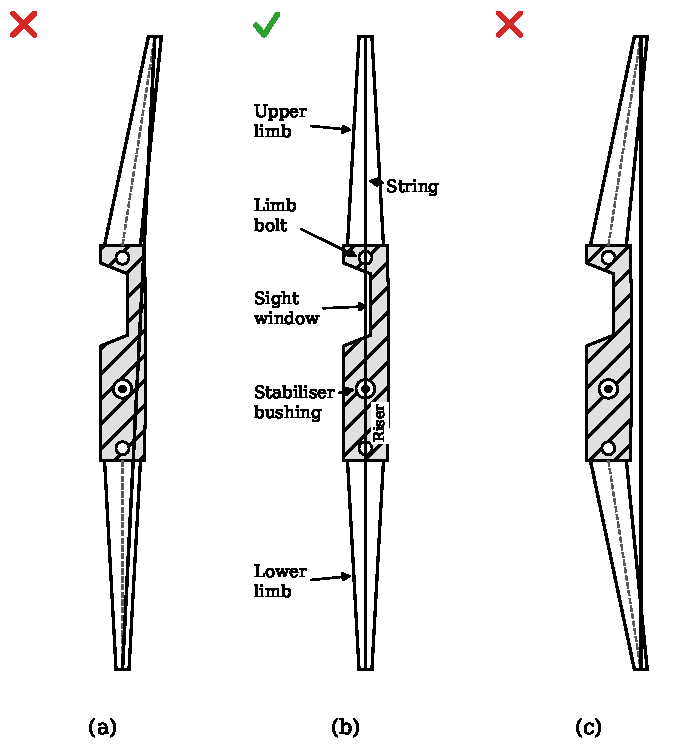
\includegraphics[width=0.6\linewidth]{limb_alignment.pdf}
  \caption{Limb alignment, viewed from behind the bow. The dashed line along each limb is the limb's centreline. (a)~Upper limb out of alignment: the string runs off-centre along the limb and misses the lower limb bolt and the stabiliser bushing. (b)~Correct: the string passes through both limb bolts and the stabiliser bushing and bisects both limbs along their length.  (c)~Both limbs out of alignment in the same direction: the string misses the bushing and both bolts. Note that this is a schematic only -- the widths of the riser and limbs, and the misalignment, are exaggerated.}
  \label{fig:limb-alignment}
\end{figure}

Before adjusting anything else, it should be checked that the limbs are correctly aligned. With the bow strung, stand behind it and sight down the string so that it lies over the limb bolts and the stabiliser bushing. When the limbs are aligned, the string should also bisect each limb along its whole length (Fig.~\ref{fig:limb-alignment}) -- sometimes limb gauges are needed to check this. If the string runs off to one side of a limb, or will not line up with the bolts and bushing at all, the limbs are out of alignment. On most modern risers this can be corrected with the lateral adjusters in the limb pockets, but doing so accurately needs a steady hand, limb-alignment gauges, and knowledge of your riser's adjustment system; it is easy to make things worse, rather than better! Unless you know what you are doing, this is something to have checked and set by an experienced archer, coach, or archery shop. It will normally have been set when you bought the bow, and it only needs revisiting if you change limbs or riser, or if the bow has had a knock.  Note that a limb which is \emph{twisted} can produce similar symptoms to misalignment, but cannot usually be corrected by adjustment; if the string sits off-centre at one limb tip no matter how the pockets are set, the limbs may need replacing.

\subsection{Draw weight}
The limb bolts set the draw weight of the bow: winding both bolts in increases it and winding them out reduces it, and most risers allow a range of a few pounds either way. Settle on your draw weight before you touch anything else, because the same bolts set the tiller and move the bracing height, so any later change of weight means re-checking everything that follows. Choose a weight you can draw and hold with good form at the end of a long session, not one you can manage for a dozen arrows when fresh; if in doubt, go lighter. Keep the bolts within the range the manufacturer allows (there is usually a stated maximum number of turns out from fully in), wind them in equal amounts so that the tiller is not disturbed, and note down how many turns out each bolt is. The weight printed on the limbs is nominal, quoted at a 28\,in draw on a 25\,in riser; what matters for choosing arrows is the weight \emph{on your fingers} at \emph{your} draw length, which can differ by several pounds. Measure it with a bow scale, or ask a coach to.

\subsection{Tiller}

\begin{figure}[htbp]
  \centering
  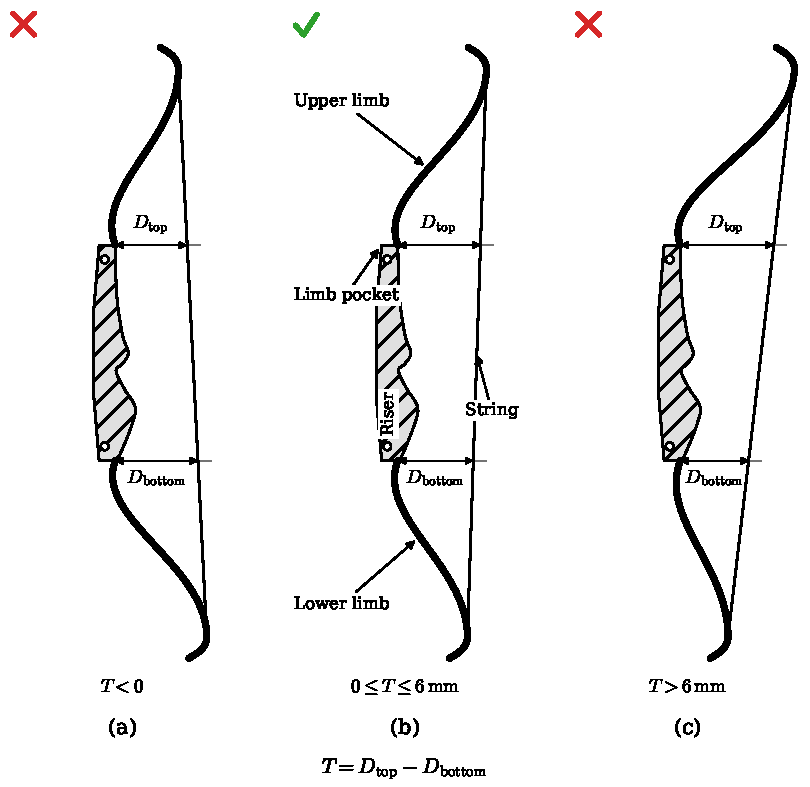
\includegraphics[width=0.7\linewidth]{tiller.pdf}
  \caption{Tiller on a recurve bow, shown via a side profile of a strung bow.  $D_\mathrm{top}$ and $D_\mathrm{bottom}$ are the perpendicular distances from the string to the point where each limb meets the riser, and the tiller is their difference, $T = D_\mathrm{top} - D_\mathrm{bottom}$. (a)~Negative tiller: the lower limb sits further from the string than the upper. (b)~Correct: between 0 and 6\,mm of positive tiller. (c)~Too much positive tiller. The asymmetry is exaggerated several-fold for clarity; a real tiller difference is a few millimetres and cannot easily be seen by eye.}
  \label{fig:tiller}
\end{figure}

Tiller is adjusted with the same limb bolts you have just used to set your draw weight, which is why it comes next; once it is set, the bolts are left alone for everything that follows. Tiller describes the balance in `pull' between the upper and lower limbs of the bow. It is measured with a bracing height gauge as the perpendicular distance from the string to the point where each limb meets the riser, taken at the top and the bottom (Fig.~\ref{fig:tiller}); the tiller is the top measurement minus the bottom. Because the arrow sits above the centre of the bow and the fingers pull unevenly on the string, most archers shoot best with a small amount of \emph{positive} tiller, meaning the top distance is slightly larger. Anywhere between 0 and 6\,mm of positive tiller is reasonable, and around 3\,mm is a sensible starting point. Winding a limb bolt \emph{in} effectively increases the `draw weight' of that limb and pulls its end of the string closer to the riser, so to increase the tiller you wind the top bolt out a little or the bottom bolt in a little. (To decrease the tiller, do the opposite.) Make small adjustments, keeping the two bolts within a quarter-turn or so of each other unless you have a reason not to, and once the tiller is in range, note it down and leave the bolts alone. If you later want to change your draw weight, wind both bolts by the same amount so the tiller is kept the same.

\subsection{Bracing height}

\begin{figure}[htbp]
  \centering
  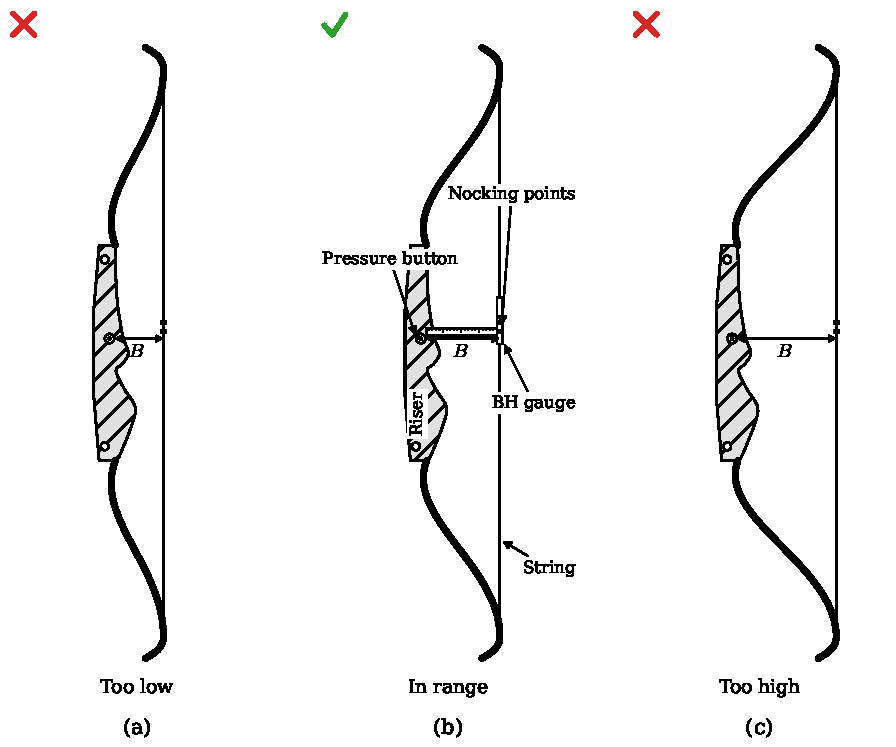
\includegraphics[width=0.8\linewidth]{bracing_height.pdf}
  \caption{Bracing height, $B$: the perpendicular distance from the string to the pressure button, measured with a bracing-height gauge clipped to the string as shown in~(b). (a)~Too low: the string sits close to the riser.  (b)~In range. (c)~Too high: the string sits far from the riser. What counts as ``in range'' depends on bow length (see text). The differences are exaggerated roughly tenfold; a bracing height that is a centimetre out does not look obviously wrong, which is why it must be measured rather than judged by eye.}
  \label{fig:bracing-height}
\end{figure}

Bracing height is the one setting every archer should know how to check and adjust. It is the perpendicular distance from the string to the pressure button (Fig.~\ref{fig:bracing-height}), and it is measured with a bracing-height gauge: clip the gauge to the string at the nocking point and read off the distance to the button. It is adjusted by twisting the string: adding twists shortens the string and raises the bracing height, removing them lowers it. As a guide, it should fall in the range 210--230\,mm for a 66\,in bow, 215--235\,mm for a 68\,in bow, and 220--240\,mm for a 70\,in bow. Within that range the exact value is not critical, but it must be the \emph{same} every time you shoot, because it affects both how your arrows fly and where your sight marks sit: a string that has lost a few twists, or stretched, will quietly move your groups. Measure it, write it down, and check it is still the same every time you string the bow. If it has dropped, add twists until it is back where it was.

\subsection{Arrows}
I classify choosing the correct arrows (length, spine, type of shaft) as part of setup. By far the most important thing here is to have an arrow that is broadly the correct length and with a spine rating that is appropriate for (i) your arrow length and (ii) your bow's \textit{measured} draw weight at your draw length. Once you know (i) and (ii), most arrow manufacturers provide a `spine chart' that will enable you to see what spine they recommend. It is often okay (and sometimes even desirable) to be one spine rating higher or lower than the chart's recommendation. If you are two or more spine ratings out, it might be time to think about buying some new arrows\ldots

Arrow length is set by your draw length. At full draw, with your bow arm and anchor where they will be once your form has settled, the back of the point should sit roughly a thumb's width in front of the rest, or a little more if you intend to use a clicker, since the clicker needs something to sit on. Beginners' draw lengths tend to grow, so err on the long side: an arrow can always be cut down but never lengthened. Check the nock fit on the string as well. The nock should click on and hold the arrow's weight when the bow is held with the arrow hanging from the string, but drop off when the string is tapped lightly. Too tight a fit slows the arrow and makes it leave erratically; too loose and the arrow can fall off at full draw. Nock fit is changed by changing the nocks or the centre serving, not by squeezing the nock.

If you shoot with a clicker, set it once your arrow length is settled: at full draw and in good alignment the blade should sit just behind the point, so that it drops off the point with the last few millimetres of expansion rather than before you have reached your anchor. Arrow length and clicker position go together, which is one more reason to settle on a length before cutting arrows down.

\subsection{Arrow rest}
Adjustment of your arrow rest controls: (i) whether your arrow is adequately supported, (ii) whether your arrow meets the pressure button at the correct vertical location, and -- consequently -- (iii) whether you have good clearance. (Here, `clearance' means that your arrows leave the bow cleanly, without interference.) See Fig.~\ref{fig:rest-position} for illustrations of how (not) to set up an arrow rest.

To set it, nock an arrow and look at the bow from behind with the string towards you, and then from the side. The height is right when the centre of the plunger button sits on the centre of the shaft; most rests have a slot or a screw that lets the arm move up and down to achieve this. The arm should extend past the centreline of the shaft but not beyond its outer edge: an arm that sticks out beyond the shaft will be struck by the fletchings, and one that stops short of the centreline will let the arrow fall off during the draw. Wire arms can be bent and trimmed to length with pliers; plastic ones are cut. Check the rest again whenever you change arrows, since a thicker or thinner shaft changes both the height and the overhang.

\begin{figure}[htbp]
  \centering
  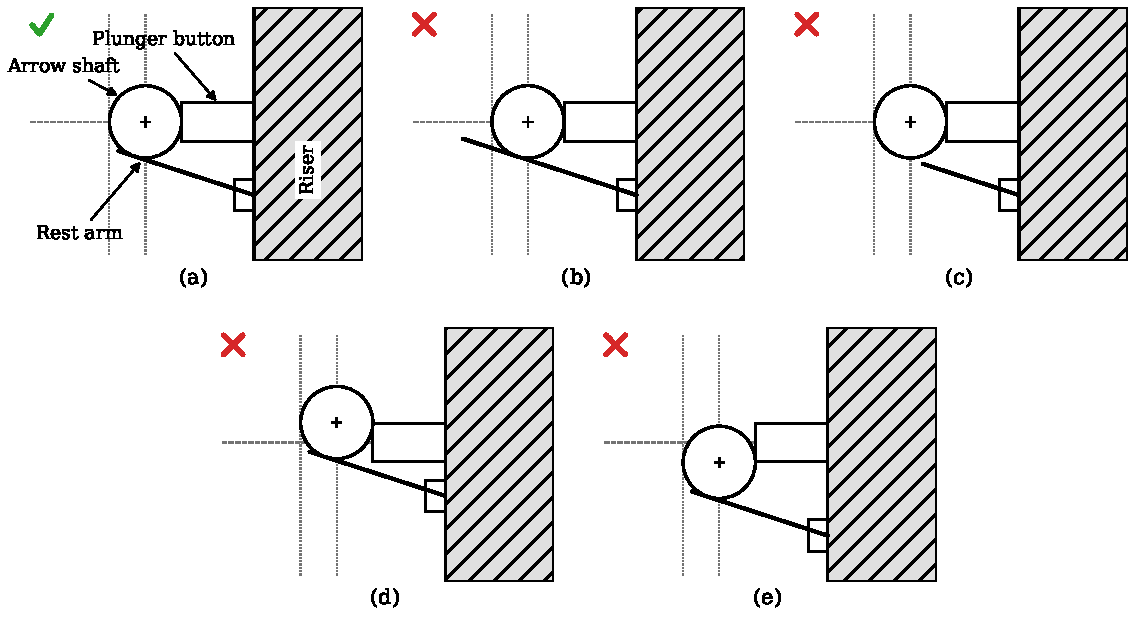
\includegraphics[width=\linewidth]{rest_position.pdf}
  \caption{Arrow rest position relative to the shaft and plunger button, viewed in cross-section from the nock end looking towards the target (right-handed bow; riser to the right of the arrow). Dashed line: plunger axis. Dotted lines: centreline and outermost extent of the shaft. (a)~Correct: the plunger pushes on the centre of the shaft, and the rest arm extends past the shaft's centreline but stops short of its outer edge. (b)~Rest arm too far out: the arm protrudes beyond the shaft. (c)~Rest arm too far in: the arm stops short of the centreline, so the arrow is barely supported and will tend to fall off during the draw. (d)~Rest too high: the plunger contacts the shaft below centre. (e)~Rest too low: the plunger contacts the shaft above centre.}
  \label{fig:rest-position}
\end{figure}

\subsection{Nocking point}
The nocking point is where the arrow sits on the string, and it is marked by two nocking points tied onto the string with serving thread, just over a nock's width apart so that the nock sits snugly between them without being pinched (Fig.~\ref{fig:nocking-point}). Brass nocking points are best avoided: they are heavy, they damage the string and tabs, and they are hard to move.  The height is checked with a bracing-height gauge clipped to the string with its arm resting on the arrow rest; the top of the lower nocking point should sit between 2 and 8\,mm above square, and 4\,mm is a good starting point if you have no reason to choose otherwise. As with bracing height, write it down and check it from time to time, because nocking points do occasionally slip or come undone. If that happens mid-session you will need to tie a new one, so it is worth learning how. There are many ways of doing this and none is better than the others; learn one that works for you and practise it at home, not on the shooting line.

\begin{figure}[htbp]
  \centering
  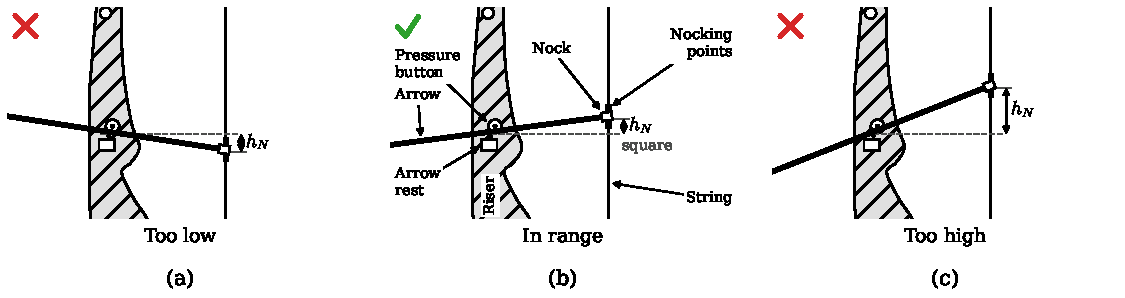
\includegraphics[width=\linewidth]{nocking_point.pdf}
  \caption{Nocking-point height, $h_N$: the height of the underside of the arrow nock (equivalently, the top of the lower nocking point) above ``square'', the line perpendicular to the string through the top of the arrow rest. Side view, string on the archer's side, limbs and grip cropped.  (a)~Too low: the nock sits at or below square and the arrow points level or slightly upwards. (b)~In range: $h_N$ between 2 and 8\,mm, so the arrow slopes very slightly downwards towards the point. (c)~Too high. The slope of the arrow is exaggerated several-fold; at a correct setting it is barely visible.}
  \label{fig:nocking-point}
\end{figure}

\subsection{Centreshot}

Centreshot is how far the arrow sits to one side or other of the bow's centreline, and it is effectively set by screwing the plunger button in or out of the riser. To check it, nock an arrow, hold the bow out at arm's length with the string towards you (or rest the bow on something), and close one eye. Line the string up so that it appears to run through the centre of both limbs (the limb bolts or limb pockets are a useful reference) and look at where the arrow point sits relative to the string (Fig.~\ref{fig:centreshot}). On a right-handed bow you should see the string passing through the point with between half and one full point width showing to the left of it; mirror this for a left-handed bow. If the point is too far out, screw the plunger in; if it is too far in, screw it out. Adjust a little at a time and re-check. Note that centreshot is a starting point rather than a precision setting: get it into the right range, note the plunger's position if you can, then leave it alone unless you have a good reason to change it.

\begin{figure}[htbp]
  \centering
  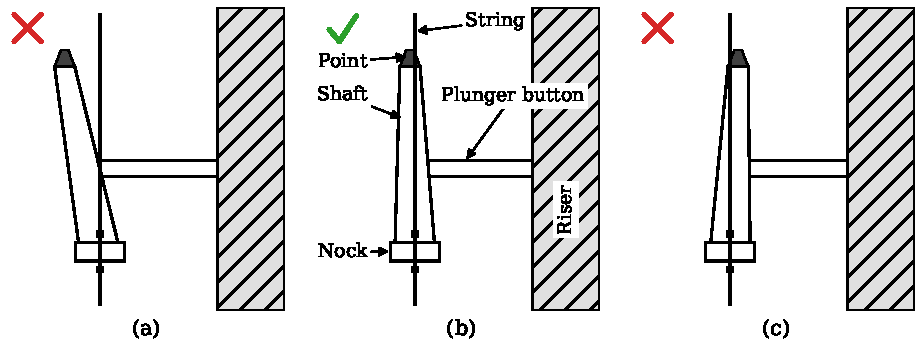
\includegraphics[width=\linewidth]{centreshot.pdf}
  \caption{Checking centreshot on a right-handed bow. The view is from behind the bow, slightly above the arrow, with the string lined up visually with the centreline of the riser and limbs. (a)~Too far out: the point sits well to the left of the string. (b)~Correct: the string passes through the point, with roughly three-quarters of the point visible to its left; anywhere between one half and one full point width is acceptable. (c)~Too far in: the point sits on or to the right of the string. Centreshot is adjusted by screwing the plunger button in or out of the riser; note how the button's visible length changes between panels.}
  \label{fig:centreshot}
\end{figure}

\subsection{Pressure button tension}
Screwing the button in and out sets the centreshot; the other thing the button controls is how firmly it pushes back on the arrow, which is set by the spring inside it. Most buttons come with two or three springs of different stiffness and a screw that adjusts the preload on whichever spring is fitted. For setup, fit the medium spring, set the adjustment to the middle of its range, and leave it there. The tension is the main thing adjusted during tuning (Section~\ref{sec:tuning}), and there is no point in fiddling with it until the rest of the setup is in range and your arrows are known to be roughly the right spine. Note the setting before you move on so that you can always get back to it.

\section{Tuning}
\label{sec:tuning}

Tuning, in the sense of Section~\ref{sec:when}, starts only once everything in Section~\ref{sec:setup} is in range. Two tests are described here, and for most club archers the first is enough. Both depend on you shooting consistently, so neither is worth attempting on a bad day.

\subsection{Bare shaft tuning}

\begin{figure}[htbp]
  \centering
  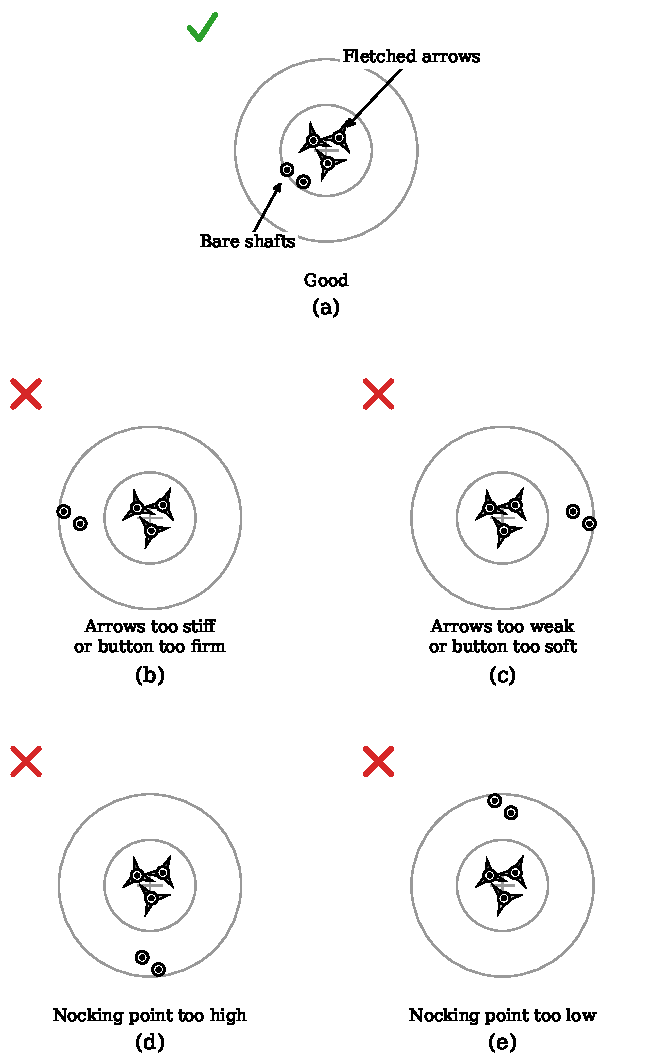
\includegraphics[width=0.9\linewidth]{bare_shaft.pdf}
  \caption{Bare-shaft tuning for a right-handed archer, viewed from the shooting line. Each panel shows a group of three fletched arrows and two bare shafts on the target. (a)~A good tune: the bare shafts land close to the fletched group, slightly low and left of it. (b)~Bare shafts to the left: the arrows are too stiff, or the pressure button is too firm. (c)~Bare shafts to the right: the arrows are too weak, or the button is too soft. (d)~Bare shafts low: the nocking point is too high. (e)~Bare shafts high: the nocking point is too low. For a left-handed archer, (b) and (c) are mirrored.}
\label{fig:bare-shaft}
\end{figure}

Bare-shaft tuning is the simplest useful test of whether your arrows match your bow. Take two or three arrows and strip the fletchings off them, or keep a couple of spare shafts unfletched for the purpose, and shoot them alongside your fletched arrows at a short distance, 18\,m indoors or 20 to 30\,m outdoors, aiming at the same point every time. A fletched arrow is steered straight by its vanes within the first few metres and lands roughly where it was aimed whatever the bow is doing; a bare shaft has nothing to correct it, so it carries the effects of any mismatch all the way to the target. Comparing the two groups therefore tells you something about the bow and arrows that the fletched group alone hides (Fig.~\ref{fig:bare-shaft}). For a right-handed archer, bare shafts landing to the left of the fletched group mean the arrows are reacting too stiffly, and bare shafts to the right mean they are reacting too weakly; both can be addressed either through the arrows (point weight, length, or ultimately spine) or through the pressure-button tension. Bare shafts landing low mean the nocking point is too high, and high means too low. A good tune is a bare-shaft group that sits close to the fletched group, slightly low and slightly left. Sort out the vertical before the horizontal, since the nocking point is quick to adjust and a wrong one confuses the left--right reading, and make one change at a time. Two warnings. First, the test only means something if you shoot consistently: a loose release or a collapsing bow arm will throw bare shafts around far more than any equipment fault, and it is easy to spend an evening ``tuning'' your form. Shoot several ends and look at where the groups sit on average, not at individual arrows. Second, in keeping with Section~\ref{sec:when}, the aim is to get into the right region, not to chase perfection; once the bare shafts are landing close to the fletched group, stop, write down what you changed, and go back to practising.

\subsection{Walk-back tuning}

\begin{figure}[htbp]
  \centering
  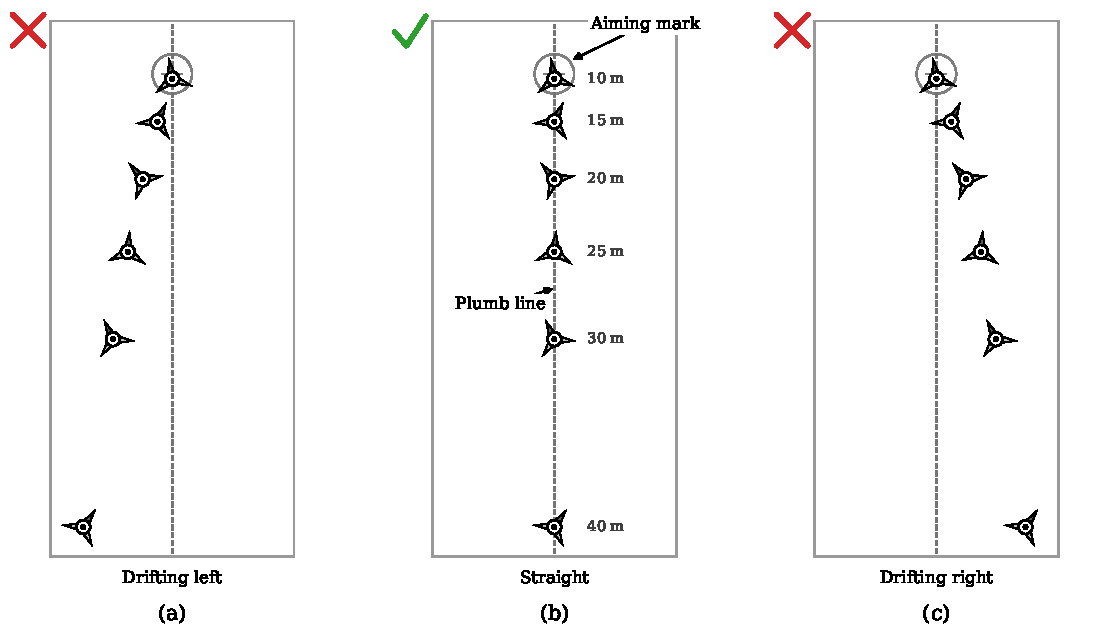
\includegraphics[width=\linewidth]{walkback.pdf}
  \caption{Walk-back tuning for a right-handed archer. With the sight set for the shortest distance, the archer aims at a mark near the top of the target from each distance in turn, so the arrows walk down the face as the distance increases. (a)~Arrows drifting left with distance: the arrows are reacting slightly stiff; soften the pressure button. (b)~Arrows falling on a vertical line below the mark: well tuned. (c)~Arrows drifting right with distance: the arrows are reacting slightly weak; stiffen the button. One arrow is drawn per distance for clarity; in practice shoot a group at each. For a left-handed archer, (a) and (c) are mirrored.}
  \label{fig:walkback}
\end{figure}

Walk-back tuning is a finer check of the pressure button once bare-shaft tuning has got you into the right region, and it is most useful outdoors where there is room. Set your sight for a short distance, say 10\,m, and fix an aiming mark near the top of the target face; a small sticker or a drawn cross is fine. Then shoot an end at the mark from 10\,m, walk back five metres, shoot another end at the same mark with the same sight setting, and so on out to 30 or 40\,m. Because the sight is not moved, each end lands lower than the last, and if the button is well matched to the arrows the groups fall on a vertical line directly below the mark (Fig.~\ref{fig:walkback}). If the line leans, the button is a little off.  For a right-handed archer, groups that drift to the left as the distance grows indicate that the arrows are reacting slightly stiff, and the button should be softened; groups that drift to the right indicate a slightly weak reaction, and the button should be stiffened. Change the tension a small amount at a time and repeat the whole sequence, since a single end at one distance tells you nothing. As with bare-shaft tuning, judge the centres of groups rather than individual arrows, keep your form honest, and stop once the line is straight enough that you would struggle to say which way it leaned; a few millimetres of lean at 40\,m is well inside the scatter of a club archer's groups and is not worth another evening.

\section{Maintenance and regular tasks}
\label{sec:maintenance}

The settings above do not stay put. Strings stretch and lose twists, screws loosen, nocking points slip and clickers creep. The checks below take a few minutes and are worth running every few weeks, and always after travelling with the bow or after a knock.

\subsection{Sight marks}
You will need to set your sight at different heights for different distances. This matters most outdoors, where we shoot a wide range of distances. The position at which you need to set your sight will also move as your technique changes and as alterations are made to your bow. You should therefore \textbf{write down} where you set your sight for a given distance, and do so on a regular basis; the recorded position is called a \textbf{sight mark}.

\subsection{Checking your clicker}
A clicker is a thin strip of metal held on by a single screw, and it moves. Check its position regularly: it creeps after a knock in a bow case or on a stand, the blade bends if an arrow is drawn through it carelessly, and your draw length lengthens as your technique improves, in which case the clicker needs to move forward with it. If your arrows start clicking early or late for no obvious reason, check the clicker before you blame anything else. Mark its position on the riser with a pencil line or a strip of tape so that any change is obvious.

\subsection{Waxing your string}
String waxing serves a few purposes: it helps bond the strands of your string together, it helps waterproof the string, and it prolongs the string's life. You need string wax, your string, your bow, and a short length of serving thread. String the bow and apply a thin layer of wax from the tube along the string, keeping it off the served sections. Then rub the wax into the string with your fingers; they should get warm but not hot, and the warmth helps the wax penetrate the fibres. Finally, wrap the serving thread once around the string, pull it fairly tight, and draw it down the string to remove the excess wax. The string should end up nice and round, shiny, and waterproof.

\subsection{Checking your string}
Measure the bracing height every time you string the bow and compare it with the figure you wrote down; if it has dropped, add twists until it is back. While the string is in your hands, look at it. The serving at the centre and at the loops should be tight and unbroken; serving that has separated so that the strands show through, or that slides along the string, needs re-serving or the string replacing. Look for fuzzy or broken strands, especially where the string meets the limb tips and around the nocking points. A string with a broken strand is finished and should not be shot. Strings are cheap compared with limbs, and one that is shot regularly is usually due for replacement after a season or so. Keep a spare, shot in and with its bracing height and nocking point set to match, so that a failure at a competition is an inconvenience rather than the end of your day.

\subsection{Checking screws and bolts}
Everything bolted to a riser works loose eventually: sight block and extension, button locking ring, rest, clicker, stabilisers and weights, and the limb bolts themselves. Every few weeks, go round every screw with the right Allen key and check that it is snug. Snug means firm, not tight: risers are aluminium and threads strip. Pay particular attention to the button's locking ring, because if it loosens the button can screw itself in or out and move your centreshot without you noticing, and to the limb bolts, which should still be at the number of turns you recorded. A drop of removable thread-lock on a screw that repeatedly loosens is acceptable; glue is not.

\subsection{Checking your arrows}
Before each session, run a thumb and finger along each shaft to feel for dents or bends, and spin each arrow on its point on a hard surface to check that it runs true; a wobbling arrow is bent or has a loose point, and either way it will not group with the others. Check that each point is firmly seated, that the nock is not cracked (a cracked nock can split on release and send the arrow anywhere), and that the fletchings are all present and stuck down along their whole length. A carbon shaft that has taken a hard hit, for instance from another arrow, should be flexed gently and listened to; any crackle means the shaft is damaged and should be binned, not shot.

\section*{Declaration on use of generative AI}
This document was prepared with the assistance of Claude Fable 5.1 (Anthropic), a large language model (LLM). The LLM assisted with production of figures and generation/refinement of portions of the text. I proofread and edited the output, and take full responsibility for the information presented here.

\section*{Licence}
\copyright{} 2026 Christopher Woodgate. This handout, including its figures, is licensed under a Creative Commons Attribution-ShareAlike 4.0 International licence (CC BY-SA 4.0): you may copy and adapt it for any purpose, provided you credit the author and share any adaptation under the same terms. See \url{https://creativecommons.org/licenses/by-sa/4.0/}. The scripts that generate the figures are licensed separately under the MIT License.

\clearpage
\section*{Setup record}
Write your settings here when you set the bow up, and check against them when something feels wrong. Measure draw weight on the fingers at your own draw length. Keep your sight marks in your scorebook, where you will have them on the line.

\medskip
\noindent Bow: \rule{5cm}{0.4pt} \hfill Date: \rule{3cm}{0.4pt}

\medskip
\renewcommand{\arraystretch}{2.2}
\noindent\begin{tabular}{|p{5.6cm}|p{3.6cm}|p{6.4cm}|}
\hline
\textbf{Setting} & \textbf{Value} & \textbf{Notes} \\ \hline
Riser and limbs (nominal weight) & & \\ \hline
Draw weight on the fingers & & \\ \hline
Limb bolts, turns out (top / bottom) & & \\ \hline
Tiller & & \\ \hline
Bracing height & & \\ \hline
Nocking point height & & \\ \hline
Button: spring and tension setting & & \\ \hline
Centreshot (button turns in) & & \\ \hline
Clicker position & & \\ \hline
Arrows: shaft, spine, length, point & & \\ \hline
\end{tabular}

\renewcommand{\arraystretch}{1}

\end{document}
